\documentclass{article}

\usepackage{times}
\usepackage{geometry}
\geometry{a4paper,left=0.6cm,right=0.7cm,top=1.5cm,bottom=1cm,columnsep=0.8cm}

\usepackage{fontawesome}          % icônes de base seulement
\usepackage[hidelinks]{hyperref}
\usepackage{multicol}
\usepackage{tikz}
\usepackage{hyphsubst}
\usepackage{moresize}
\usepackage{hyphenat}
\usepackage{tabularx}
\usepackage{ragged2e}
\usepackage{xcolor}
\usepackage{enumitem}
\usetikzlibrary{calc, positioning}
\newcolumntype{Y}{>{\RaggedRight\arraybackslash}X}

% icônes manquantes -> puce
\makeatletter
\@for\sym:=faBrain,faMicrochip,faHandshakeO,faTools,faNetworkWired,%
             faDatabase,faServer,faGit,faUsers,faComments,faCalendar,faGroup\do{%
  \@ifundefined{\sym}{\expandafter\newcommand\csname\sym\endcsname{\textbullet}}{}}
\makeatother

% couleurs
\definecolor{maincolor}{HTML}{f0fafc}
\definecolor{seccolor}{HTML}{ffffff}
\definecolor{gray}{HTML}{8c94a9}
\definecolor{sidetext}{HTML}{59cee5}

% bande latérale bleue
\usepackage{eso-pic}
\AddToShipoutPictureBG{%
  \begin{tikzpicture}[remember picture,overlay]
    \fill[maincolor] (current page.north west) rectangle
                     ([xshift=0.3\paperwidth] current page.south west);
  \end{tikzpicture}%
}

% listes
\setlist[itemize]{itemsep=-2pt,topsep=0pt,leftmargin=1.08cm}
\renewcommand{\labelitemi}{\textcolor{sidetext}{\footnotesize$\bullet$}}

\setlength{\parindent}{0pt}
\usepackage{paracol}
\columnratio{0.3}

\begin{document}
\pagestyle{empty}

\begin{paracol}{2}
% ────────────────────────────────────────
% Colonne gauche
% ────────────────────────────────────────
\color{sidetext}
\vspace*{-0.5cm}

\noindent
\begin{minipage}{\linewidth}
  \centering
  \begin{tikzpicture}
    \clip (0,0) circle (1.5cm) node[anchor=center]
      {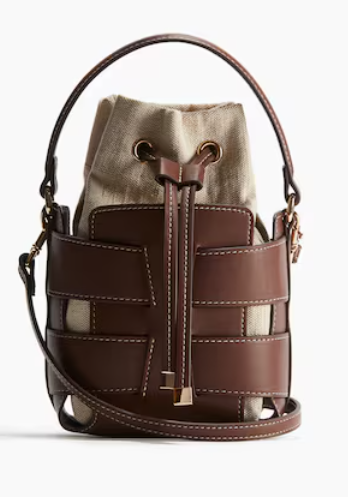
\includegraphics[width=3cm]{b902beee3872451089061da6ec386aaf.png}};
  \end{tikzpicture}

  \vspace{3mm}
  {\color{black}\LARGE \textbf{Judikael Mourouvin}}

  \vspace{1mm}
  {\large Technicien informatique \& marketing digital}

  \vspace{3mm}
  {\color{gray}\rule{\linewidth}{0.4pt}} \\
\end{minipage}

% ── Coordonnées
\begin{tabular}{@{}c l}
  \faPhone &
  \begin{tabular}[t]{@{}l@{}}
    {\color{gray}Téléphone} \\ +590 0690 91 14 48
  \end{tabular} \\
  \\
  \faLinkedin &
  \begin{tabular}[t]{@{}l@{}}
    {\color{gray}LinkedIn} \\
    \href{}{Mon LinkedIn}
  \end{tabular} \\
  \\
  \faMapMarker &
  \begin{tabular}[t]{@{}l@{}}
    {\color{gray}Adresse} \\ Route de Cocoyer \\ 97190 Gosier
  \end{tabular} \\
  \\
  \faEnvelope &
  \begin{tabular}[t]{@{}l@{}}
    {\color{gray}Email} \\
    \href{mailto:jkmou971@gmail.com}{jkmou971@gmail.com}
  \end{tabular} \\
\end{tabular}

\vspace{2mm}
{\color{gray}\rule{\linewidth}{0.4pt}} \\

% ── Langues --------------------------------------------------------
{\color{black}{Langues}}

\vspace{2mm}
\begin{itemize}[leftmargin=*]
\item Anglais - \textcolor{gray}{}
\item Espagnol - \textcolor{gray}{}\end{itemize}          % ← le placeholder va contenir \begin{itemize}…\end{itemize}

{\color{gray}\rule{\linewidth}{0.4pt}} \\

% ── Compétences ----------------------------------------------------
\vspace{2mm}
{\color{black}{Compétences Clés}}

\vspace{2mm}
\begin{itemize}[leftmargin=*]
\item Marketing
\item Réseaux
\item Support
\item Maintenance
\item Diagnostic
\item Administration
\item Configuration\end{itemize}              % ← idem, une vraie liste
\vspace{2mm}
{\color{gray}\rule{\linewidth}{0.4pt}} \\

% ── Centres d'intérêt
\vspace{2mm}
{\color{black}{Centres d’intérêt}}

\vspace{2mm}
\begin{itemize}[leftmargin=*]
\item Lectur
\item Sports
\item Musique
\item Voyage
\end{itemize}     % ← simple itemize ou tabular

\vfill
~

% ────────────────────────────────────────
\switchcolumn
% Colonne droite
% ────────────────────────────────────────
\color{black}

% ── Profil
\textcolor{black}{\Large \textbf{Profil Professionnel}} \\[2pt]
Passionné par l’informatique et le marketing digital, j’ai développé de solides compétences en configuration de postes, maintenance et support utilisateur. Après une année d’alternance à la DSI de la Mairie du Gosier, je souhaite poursuivre à temps plein pour accompagner vos projets numériques. Polyvalent et rigoureux, je maîtrise la gestion de réseaux, l’assistance technique et la mise en place de stratégies digitales. Mon objectif : apporter efficacité et réactivité aux équipes tout en améliorant l’expérience utilisateur. \\[8pt]

% ── Expérience
\textcolor{black}{\Large \textbf{Expérience Professionnelle}} \\[2pt]

\colorbox{maincolor}{%
  \begin{minipage}{\linewidth}
    \textbf{Alternant en Marketing Digital}   2023-2024  \\ Mairie du Gosier – DSI 
    \begin{itemize}
      \item Géré des projets numériques pour moderniser les services municipaux \item Analysé les besoins des agents et déployé des solutions adaptées \item Assuré le support et formé les utilisateurs pour accroître leur autonomie \item Contribué aux actions de marketing digital afin de renforcer la visibilité
    \end{itemize}
  \end{minipage}}

\vspace{3mm}


\colorbox{maincolor}{%
  \begin{minipage}{\linewidth}
    \textbf{Animateur de la zone informatique}   2022-2023  \\ Pôle Emploi, Gosier 
    \begin{itemize}
      \item Fournit assistance et support technique aux demandeurs d’emploi \item Configuré et entretenu les postes de travail pour garantir leur fiabilité \item Diagnostiqué et résolu les incidents afin de minimiser les interruptions
    \end{itemize}
  \end{minipage}}

\vspace{3mm}


\colorbox{maincolor}{%
  \begin{minipage}{\linewidth}
    \textbf{Stagiaire Informaticien}   2020-2021  \\ Numerika, Baie-Mahault 
    \begin{itemize}
      \item Configuré et maintenu les équipements informatiques du parc \item Assuré le support utilisateur pour optimiser la continuité de service
    \end{itemize}
  \end{minipage}}   % ← blocs \colorbox{maincolor}{\begin{minipage}…}

\vspace{8mm}

% ── Formation
\textcolor{black}{\Large \textbf{Formation}} \\[2pt]

\begin{tabularx}{\linewidth}{@{}c  >{\RaggedRight\arraybackslash}X
                             >{\raggedleft\arraybackslash}p{0.25\linewidth}@{}}
\textcolor{sidetext}{\faGraduationCap} &
Bachelor Marketing Digital &
2023-2024 \\
& CFA IUTS & \\   % ligne de l’établissement
\end{tabularx}
\begin{itemize}[leftmargin=*]
  \item Stratégies de communication digitale et gestion de campagne
  \item Analyse de données marketing et optimisation de la performance
  \item Gestion de projet numérique et réseaux sociaux
\end{itemize}
\vspace{3mm}

\begin{tabularx}{\linewidth}{@{}c  >{\RaggedRight\arraybackslash}X
                             >{\raggedleft\arraybackslash}p{0.25\linewidth}@{}}
\textcolor{sidetext}{\faGraduationCap} &
BTS Systèmes Numériques option Informatique et Réseaux &
2019-2021 \\
& Lycée Chevalier Saint-Georges, Abymes & \\   % ligne de l’établissement
\end{tabularx}
\begin{itemize}[leftmargin=*]
  \item Administration de réseaux locaux et sécurité informatique
  \item Maintenance matérielle et logicielle de systèmes connectés
  \item Support technique et gestion d’incidents
\end{itemize}       % ← lignes tabular par diplôme

\end{paracol}
\end{document}

